\documentclass{beamer}

\usepackage{graphicx}
\graphicspath{ {./images/} }

%\usetheme{Madrid}
\usetheme{Warsaw}

\title[Logistical Optimisation for Offshore Windfarms]{Simulation and Optimisation of Offshore Renewable Energy Arrays for Minimal Life-Cycle Costs}

\author{R. Kuipers}

\date{October 10, 2019}

\begin{document}

\begin{frame}
  \titlepage
\end{frame}

\begin{frame}{The problem}
  \begin{itemize}
  	\item Focus on modern windfarms in the North Sea, relatively far from the coast, 100+ wind turbines, lifespan of about 20-30 years, costs of installation in range of \pounds 100 million or higher
  	\item Optimize logistics of operations on offshore windfarms (OWFs) in each phase of the life-cycle:
  	\begin{itemize}
  		\item Installation
  		\item Maintenance
  		\item Decommission
  	\end{itemize}
  	\item Logisitical descisions consists of layout, vessel scheduling, routing, number and types of vessels
  	\item Small optimisations can have significant effects on costs, as vessels can cost upwards of \pounds 100,000 per day
  	\item Methods used are optimisation and simulation
  \end{itemize}
\end{frame}


\begin{frame}{Key challenges}
  \begin{itemize}
  	\item Long lead up for many decisions means no last-minute scheduling
  	\item Maritime weather conditions can be unpredictable
  	\item Looking at the whole life-cycle includes a lot of different types of decisions
  	\item Location-specific circumstances can have a big effect on weather conditions and duration of tasks
  	\item Phases are not independent, maintenance starts at the same time installation starts
  \end{itemize}
\end{frame}


\begin{frame}{Existing literature}
   \begin{itemize}
  	\item Various attempts to improve the installation phase, through integer programming and local search, combined with simulation
  	\item A lot of research has been done in various areas of maintenance, including supply chain management, mitigating failure rate, condition based maintenance
  	\item Not a lot of research has been done on decommission projects, but they are similar in structure to installation projects
  	\item No research at all has been found that looks at the entire life-cycle and how the different phases affect each other
  \end{itemize}
\end{frame}


\begin{frame}{Current Progress}
   \begin{itemize}
  	\item Reviewed a large part of the literature, primarily on installation projects and secondarily on maintenance projects and general non-deterministic scheduling and logistics
  	\item Laid the foundations for a decision support tool suited to analyse and optimise schedules for any phase of the life-cycle, based on site-specific characteristics of the project
  	\item Planned the interactions between my various models	
  \end{itemize}
\end{frame}


\begin{frame}{Model interactions}
\begin{figure}[t]
  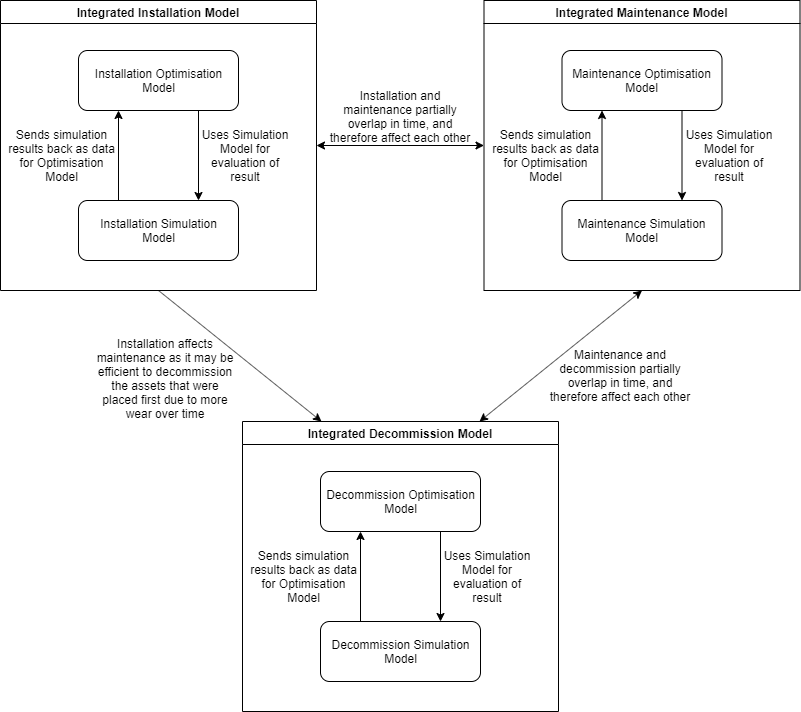
\includegraphics[width=0.8\textwidth]{flowchart}
\centering
\end{figure}
\end{frame}


\begin{frame}{Future Work}
   \begin{itemize}
  	\item Develop full models for each stage of the life-cycle
  	\item Determine specific interactions between the stages
  	\item Implement models in the tool, develop it further for full commercial functionality
  	\item Validate and test the tool (and underlying models) using real data
  \end{itemize}
\end{frame}

\end{document}


